\chapter{An Application Example (Out of Date)}\label{ch-appl-example}
\thispagestyle{headings}
\markboth{Chapter \ref{ch-appl-example}: An Application Example}{Chapter \ref{ch-appl-example}: An Application Example}

%The QUESO-MCMC Tool currently implements the DRAM algorithm \cite{HaLaMiSa06} for the generation of a Markov chain.
%Section \ref{sc-appl-run-eight-steps} explains how to develop your own application using the DRAM capabilities of the QUESO-MCMC Tool, while
%Section \ref{sc-appl-run-dram-output} describes the output information generated by the toolkit and
%Sections
%\ref{sc-appl-run-dram-normal-ex},
%\ref{sc-appl-run-dram-chem-ex} and
%\ref{sc-appl-run-dram-algae-ex}
%describe the three examples available,
%all of them also available in \cite{mcmctool}.

%The chapter ends at Section \ref{sc-appl-run-planned-features} with a brief list of planned features for next toolkit versions w.r.t. Markov Chain Monte Carlo methods.

\clearpage
\section{Examples of Statistical Problems}

\subsection{Statistical Inverse Problem}

In this example we have $n=2$, that is,
\begin{equation*}
\boldsymbol{\theta} = 
\left(
\begin{array}{c}
\theta_1 \\
\theta_2
\end{array}
\right)\in \mathbb{R}^2.
\end{equation*}
Also, 
\begin{equation*}
\pi_{\text{prior}}(\boldsymbol{\theta}) \varpropto 1
\end{equation*}
and
\begin{equation*}
\pi_{\text{like}}(\boldsymbol{\theta}) \varpropto e^{-\frac{1}{2}\left\{(\boldsymbol{\theta}-\boldsymbol{\mu})^T[\mathbf{C}^{-1}](\boldsymbol{\theta}-\boldsymbol{\mu})\right\}},
\end{equation*}
with
\begin{equation}\label{eq-example-mu}
\boldsymbol{\mu} = 
\left(
\begin{array}{c}
-1 \\
2
\end{array}
\right)
\end{equation}
and
\begin{equation}\label{eq-example-cov-mat}
\mathbf{C} = 
\left[
\begin{array}{cc}
4 & 0 \\
0 & 1
\end{array}
\right].
\end{equation}
The posterior pdf is then given by
\begin{equation}\label{eq-example-post}
\pi_{\text{post}}(\boldsymbol{\theta}) \varpropto e^{-\frac{1}{2}\left\{(\boldsymbol{\theta}-\boldsymbol{\mu})^T[\mathbf{C}^{-1}](\boldsymbol{\theta}-\boldsymbol{\mu})\right\}}.
\end{equation}

It is clear that for such problem it is possible to analytically compute the exact posterior pdf as
\begin{eqnarray*}
\pi_{\text{post}}(\boldsymbol{\theta}) & = & \frac{1}{4\pi} e^{-\frac{1}{2}\left\{(\boldsymbol{\theta}-\boldsymbol{\mu})^T[\mathbf{C}^{-1}](\boldsymbol{\theta}-\boldsymbol{\mu})\right\}} \\
                                       & = & \frac{1}{4\pi} e^{-\frac{1}{8}(\theta_1+1)^2 - \frac{1}{2}(\theta_2-2)^2}, \label{eq-example-exact-joint}
\end{eqnarray*}
and to sample it through the formula
\begin{equation*}
\boldsymbol{\mu}+\mathbf{C}^{1/2}\mathcal{N}(0,I),
\end{equation*}
where $\mathcal{N}(0,I)$ designates a Gaussian joint pdf of zero mean and unit covariance matrix
and
\begin{equation*}
\mathbf{C}^{1/2} = 
\left[
\begin{array}{cc}
2 & 0 \\
0 & 1
\end{array}
\right].
\end{equation*}
Nonetheless, we will use QUESO to sample the posterior \eqref{eq-example-post}
with a Markov chain algorithm available in QUESO, and
then check the marginal results for $\theta_1$ and $\theta_2$ against the analytical formulas
\begin{eqnarray*}
\pi_{\text{post}}(\theta_1) & = & \frac{1}{2\sqrt{2\pi}} e^{-\frac{1}{8}(\theta_1+1)^2}, \label{eq-example-exact-marg-1}\\
\pi_{\text{post}}(\theta_1) & = & \frac{1}{ \sqrt{2\pi}} e^{-\frac{1}{2}(\theta_2-2)^2}. \label{eq-example-exact-marg-2}
\end{eqnarray*}

\subsection{Statistical Forward Problem}

Once the solution $\boldsymbol{\Theta}_{\text{post}}$ of the statistical inverse problem is obtained,
it is used for a statistical forward problem where $n=2$ and $m=1$, that is,
\begin{equation*}
\mathbf{q}:\mathbb{R}^2\rightarrow\mathbb{R}.
\end{equation*}
Also, we have the very simple situation
\begin{equation}\label{eq-example-q}
\mathbf{q}(\boldsymbol{\theta}) = \theta_1+\theta_2,\quad\forall\boldsymbol{\theta}\in\mathbb{R}^2.
\end{equation}
Since the solution $\mathbf{Q}$ of this statistical forward problem is the sum of
two rvs $\boldsymbol{\Theta}_1$ and $\boldsymbol{\Theta}_2$,
and since these two rvs are independent Gaussian rvs by assumption, we should have
\begin{equation}\label{eq-example-E}
E[\mathbf{Q}] = E[\boldsymbol{\Theta}_1] + E[\boldsymbol{\Theta}_2] = -1 + 2 = 1
\end{equation}
and
\begin{equation}\label{eq-example-V}
V[\mathbf{Q}] = V[\boldsymbol{\Theta}_1] + V[\boldsymbol{\Theta}_2] = 4 + 1 = 5
\end{equation}
where ``E'' and ``V'' indicate expectation and variance respectively.

\clearpage
\section{Application Code}

The program example given in this paper is compatible with version 0.41.0 of QUESO \cite{Pr09c}.
The source code for the example is composed of 7 files:
\begin{itemize}
\item example\_main.C (Figure \ref{fig-main-c}),
\item example\_likelihood.h and example\_likelihood.C (Figures \ref{fig-like-h} and \ref{fig-like-c}),
\item example\_qoi.h and example\_qoi.C (Figures \ref{fig-qoi-h} and \ref{fig-qoi-c}), and
\item example\_compute.h and example\_compute.C (Figures \ref{fig-compute-h}, \ref{fig-compute-c1} and \ref{fig-compute-c2}).
\end{itemize}
The makefile is given in Figure \ref{fig-make} and the options input file is given in Figures \ref{fig-options-input-1}, \ref{fig-options-input-2} and \ref{fig-options-input-3}.
Once the code is compiled, one just needs to run ``example\_gsl example.inp''.

\begin{figure}[h!]
\begin{center}
\begin{verbatim}
#include <example_compute.h>

int main(int argc, char* argv[])
{
  // Initialize environment
  MPI_Init(&argc,&argv);

  UQ_FATAL_TEST_MACRO(argc != 2,
                      UQ_UNAVAILABLE_RANK,
                      "main()",
                      "input file must be specified in command line
                       as argv[1], just after executable argv[0]");
  uqFullEnvironmentClass* env =
    new uqFullEnvironmentClass(MPI_COMM_WORLD,argv[1],"");

  // Compute
  compute(*env);

  // Finalize environment
  delete env;
  MPI_Finalize();

  return 0;
}
\end{verbatim}
\end{center}
\caption{
The example\_main.C file.
}
\label{fig-main-c}
\end{figure}

\begin{figure}[h!]
\begin{center}
\begin{verbatim}
#ifndef __EX_LIKELIHOOD_H__
#define __EX_LIKELIHOOD_H__

#include <uqGslMatrix.h>

struct
likelihoodRoutine_DataType
{
  const uqGslVectorClass* meanVector;
  const uqGslMatrixClass* covMatrix;
};

double likelihoodRoutine(
  const uqGslVectorClass& paramValues,
  const uqGslVectorClass* paramDirection,
  const void*             functionDataPtr,
  uqGslVectorClass*       gradVector,
  uqGslMatrixClass*       hessianMatrix,
  uqGslVectorClass*       hessianEffect);

#endif
\end{verbatim}
\end{center}
\caption{
The example\_likelihood.h file
}
\label{fig-like-h}
\end{figure}

\begin{figure}[h!]
\begin{center}
\begin{verbatim}
#include <example_likelihood.h>

double likelihoodRoutine(
  const uqGslVectorClass& paramValues,
  const uqGslVectorClass* paramDirection,
  const void*             functionDataPtr,
  uqGslVectorClass*       gradVector,
  uqGslMatrixClass*       hessianMatrix,
  uqGslVectorClass*       hessianEffect)
{
  // Just checking: the user, at the application level, expects
  // vector 'paramValues' to have size 2.
  UQ_FATAL_TEST_MACRO(paramValues.sizeGlobal() != 2,
                      UQ_UNAVAILABLE_RANK,
                      "likelihoodRoutine()",
                      "paramValues vector does not have size 2");

  // This code exemplifies multiple Metropolis-Hastings solvers, each calling
  // this likelihood routine.
  //
  // In this simple example, only node 0 in each subenvironment does the job
  // even though there might be more than one node per subenvironment.
  // In a more realistic situation, if the user is asking for multiple nodes per
  // subenvironment, then the model code in the qoi and likelihood routines
  // might really demand more than one node.
  //
  // Here we use 'env.subRank()' only. A realistic application might want to use
  // 'env.subComm()' or 'env.subComm().Comm()'
  double result = 0.;
  const uqBaseEnvironmentClass& env = paramValues.env();
  if (env.subRank() == 0) {
    const uqGslVectorClass& meanVector =
      *((likelihoodRoutine_DataType *) functionDataPtr)->meanVector;
    const uqGslMatrixClass& covMatrix  =
      *((likelihoodRoutine_DataType *) functionDataPtr)->covMatrix;

    uqGslVectorClass diffVec(paramValues - meanVector);

    result = scalarProduct(diffVec, covMatrix.invertMultiply(diffVec));
  }
  else {
    // Do nothing;
  }

  return -.5*result;
}
\end{verbatim}
\end{center}
\caption{
The example\_likelihood.C file
}
\label{fig-like-c}
\end{figure}

\begin{figure}[h!]
\begin{center}
\begin{verbatim}
#ifndef __EX_QOI_H__
#define __EX_QOI_H__

#include <uqGslMatrix.h>
#include <EpetraExt_DistArray.h>

struct
qoiRoutine_DataType
{
  double coef1;
  double coef2;
};

void
qoiRoutine(
  const uqGslVectorClass&                        paramValues,
  const uqGslVectorClass*                        paramDirection,
  const void*                                    functionDataPtr,
        uqGslVectorClass&                        qoiValues,
        EpetraExt::DistArray<uqGslVectorClass*>* gradVectors,
        EpetraExt::DistArray<uqGslMatrixClass*>* hessianMatrices,
        EpetraExt::DistArray<uqGslVectorClass*>* hessianEffects);

#endif
\end{verbatim}
\end{center}
\caption{
The example\_qoi.h file
}
\label{fig-qoi-h}
\end{figure}

\begin{figure}[h!]
\begin{center}
\begin{verbatim}
#include <example_qoi.h>
void qoiRoutine(
  const uqGslVectorClass&                        paramValues,
  const uqGslVectorClass*                        paramDirection,
  const void*                                    functionDataPtr,
        uqGslVectorClass&                        qoiValues,
        EpetraExt::DistArray<uqGslVectorClass*>* gradVectors,
        EpetraExt::DistArray<uqGslMatrixClass*>* hessianMatrices,
        EpetraExt::DistArray<uqGslVectorClass*>* hessianEffects)
{
  // Just checking: the user, at the application level, expects
  // vector 'paramValues' to have size 2 and
  // vector 'qoiValues' to have size 1.
  UQ_FATAL_TEST_MACRO(paramValues.sizeGlobal() != 2,
                      UQ_UNAVAILABLE_RANK,
                      "qoiRoutine()",
                      "paramValues vector does not have size 2");
  UQ_FATAL_TEST_MACRO(qoiValues.sizeGlobal() != 1,
                      UQ_UNAVAILABLE_RANK,
                      "qoiRoutine()",
                      "qoiValues vector does not have size 1");

  // This code exemplifies multiple Monte Carlo solvers, each calling this
  // qoi routine.
  //
  // In this simple example, only node 0 in each subenvironment does the job
  // even though there might be more than one node per subenvironment.
  // In a more realistic situation, if the user is asking for multiple nodes per
  // subenvironment, then the model code in the qoi and likelihood routines
  // might really demand more than one node.
  //
  // Here we use 'env.subRank()' only. A realistic application might want to use
  // 'env.subComm()' or 'env.subComm().Comm()'
  const uqBaseEnvironmentClass& env = paramValues.env();
  if (env.subRank() == 0) {
    double coef1 = ((qoiRoutine_DataType *) functionDataPtr)->coef1;
    double coef2 = ((qoiRoutine_DataType *) functionDataPtr)->coef2;
    qoiValues[0] = (coef1*paramValues[0] + coef2*paramValues[1]);
  }
  else {
    qoiValues[0] = 0.;
  }
  return;
}
\end{verbatim}
\end{center}
\caption{
The example\_qoi.C file
}
\label{fig-qoi-c}
\end{figure}

\begin{figure}[h!]
\begin{center}
\begin{verbatim}
#ifndef __EX_COMPUTE_H__
#define __EX_COMPUTE_H__

#include <uqEnvironment.h>

void compute(const uqFullEnvironmentClass& env);

#endif
\end{verbatim}
\end{center}
\caption{
The example\_compute.h file
}
\label{fig-compute-h}
\end{figure}

\begin{figure}[h!]
\begin{center}
\begin{verbatim}
#include <example_compute.h>
#include <example_likelihood.h>
#include <example_qoi.h>
#include <uqGslMatrix.h>
#include <uqStatisticalInverseProblem.h>
#include <uqStatisticalForwardProblem.h>

void compute(const uqFullEnvironmentClass& env) {
  // Step 1 of 9: Instantiate the parameter space
  uqVectorSpaceClass<uqGslVectorClass,uqGslMatrixClass>
    paramSpace(env, "param_", 2, NULL);

  // Step 2 of 9: Instantiate the parameter domain
  uqGslVectorClass paramMins(paramSpace.zeroVector());
  paramMins.cwSet(-INFINITY);
  uqGslVectorClass paramMaxs(paramSpace.zeroVector());
  paramMaxs.cwSet( INFINITY);
  uqBoxSubsetClass<uqGslVectorClass,uqGslMatrixClass>
    paramDomain("param_",paramSpace,paramMins,paramMaxs);

  // Step 3 of 9: Instantiate the likelihood function object
  uqGslVectorClass meanVector(paramSpace.zeroVector());
  meanVector[0] = -1;
  meanVector[1] =  2;
  uqGslMatrixClass covMatrix(paramSpace.zeroVector());
  covMatrix(0,0) = 4.; covMatrix(0,1) = 0.;
  covMatrix(1,0) = 0.; covMatrix(1,1) = 1.;
  likelihoodRoutine_DataType likelihoodRoutine_Data;
  likelihoodRoutine_Data.meanVector = &meanVector;
  likelihoodRoutine_Data.covMatrix  = &covMatrix;
  uqGenericScalarFunctionClass<uqGslVectorClass,uqGslMatrixClass>
    likelihoodFunctionObj("like_",
                          paramDomain,
                          likelihoodRoutine,
                          (void *) &likelihoodRoutine_Data,
                          true); // routine computes [ln(function)]

  // Step 4 of 9: Instantiate the inverse problem
  uqUniformVectorRVClass<uqGslVectorClass,uqGslMatrixClass>
    priorRv("prior_", paramDomain);
  uqGenericVectorRVClass<uqGslVectorClass,uqGslMatrixClass>
    postRv("post_", paramSpace);
  uqStatisticalInverseProblemClass<uqGslVectorClass,uqGslMatrixClass>
    ip("", priorRv, likelihoodFunctionObj, postRv);
\end{verbatim}
\end{center}
\caption{
Initial part of example\_compute.C file: the first 4 of the 5 steps to deal with the statistical inverse problem.
}
\label{fig-compute-c1}
\end{figure}

\begin{figure}[h!]
\begin{center}
\begin{verbatim}
  // Step 5 of 9: Solve the inverse problem
  uqGslVectorClass paramInitials(paramSpace.zeroVector());
  paramInitials[0] = 0.1;
  paramInitials[1] = -1.4;
  uqGslMatrixClass proposalCovMatrix(paramSpace.zeroVector());
  proposalCovMatrix(0,0) = 8.; proposalCovMatrix(0,1) = 4.;
  proposalCovMatrix(1,0) = 4.; proposalCovMatrix(1,1) = 16.;
  ip.solveWithBayesMetropolisHastings(paramInitials, &proposalCovMatrix);

  // Step 6 of 9: Instantiate the qoi space
  uqVectorSpaceClass<uqGslVectorClass,uqGslMatrixClass>
    qoiSpace(env, "qoi_", 1, NULL);

  // Step 7 of 9: Instantiate the qoi function object
  qoiRoutine_DataType qoiRoutine_Data;
  qoiRoutine_Data.coef1 = 1.;
  qoiRoutine_Data.coef2 = 1.;
  uqGenericVectorFunctionClass<uqGslVectorClass,uqGslMatrixClass,
                               uqGslVectorClass,uqGslMatrixClass>
    qoiFunctionObj("qoi_",
                   paramDomain,
                   qoiSpace,
                   qoiRoutine,
                   (void *) &qoiRoutine_Data);

  // Step 8 of 9: Instantiate the forward problem
  uqGenericVectorRVClass<uqGslVectorClass,uqGslMatrixClass>
    qoiRv("qoi_", qoiSpace);
  uqStatisticalForwardProblemClass<uqGslVectorClass,uqGslMatrixClass,
                                   uqGslVectorClass,uqGslMatrixClass>
    fp("", postRv, qoiFunctionObj, qoiRv);

  // Step 9 of 9: Solve the forward problem
  fp.solveWithMonteCarlo();

  return;
}
\end{verbatim}
\end{center}
\caption{
Final part of example\_compute.C file: the final step of the 5 steps to deal with the statistical inverse problem and the 4 steps to deal with the statistical forward problem.
}
\label{fig-compute-c2}
\end{figure}

\clearpage
\section{Application Compilation}

\begin{figure}[h!]
\begin{center}
\begin{verbatim}
QUESO_DIR = /basepath/Installations/queso_0_41_0_gnu/
TRILINOS_DIR = /basepath/Installations/Trilinos_8_0_7/
BOOST_DIR = /basepath/Installations/Boost_1_35_0/
HPCT_DIR = /org/centers/pecos/LIBRARIES/hpct/0.25.1/
include $(TRILINOS_DIR)/include/Makefile.export.epetra

INC_PATHS = \
        -I. \
        -I$(QUESO_DIR)/include \
        -I$(MPI_DIR)/include \
        -I$(BOOST_DIR)/include/boost-1_35 \
        -I$(GSL_DIR)/include \
        -I$(HPCT_DIR)/include \
        $(EPETRA_INCLUDES)

LIBS = \
        -L$(QUESO_DIR)/lib -lqueso \
        -L$(MPI_DIR)/lib \
        -L$(TRILINOS_DIR)/lib \
        -L$(BOOST_DIR)/lib -lboost_program_options \
        -L$(GSL_DIR)/lib -lgsl \
        -L$(HPCT_DIR)/lib -lhpct \
        $(EPETRA_LIBS)

CXX = mpicxx
CXXFLAGS += -O3 -Wall -c

default: all

.SUFFIXES: .o .C

all:    ex_gsl

clean:
        rm -f *~
        rm -f *.o
        rm -f example

ex_gsl: example_main.o example_likelihood.o example_qoi.o example_compute.o
        $(CXX) example_main.o example_likelihood.o example_qoi.o example_compute.o \
               -o example_gsl $(LIBS)

%.o: %.C
        $(CXX) $(INC_PATHS) $(CXXFLAGS) $<
\end{verbatim}
\end{center}
\caption{
Makefile for the program in Figures \ref{fig-main-c}-\ref{fig-compute-c2}.
}
\label{fig-make}
\end{figure}

\clearpage
\section{Application Input File}

\begin{figure}[h!]
\begin{center}
\begin{verbatim}
###############################################
# UQ Environment
###############################################
#env_help                = anything
env_numSubEnvironments   = 1
env_subDisplayFileName   = outputData/display
env_subDisplayAllowAll   = 0
env_subDisplayAllowedSet = 0
env_displayVerbosity     = 2
env_syncVerbosity        = 0
env_seed                 = 0

###############################################
# Statistical inverse problem (ip)
###############################################
#ip_help                 = anything
ip_computeSolution      = 1
ip_dataOutputFileName   = outputData/sipOutput
ip_dataOutputAllowedSet = 0

###############################################
# Statistical forward problem (fp)
###############################################
fp_help                 = anything
fp_computeSolution      = 1
fp_computeCovariances   = 1
fp_computeCorrelations  = 1
fp_dataOutputFileName   = outputData/sfpOutput
fp_dataOutputAllowedSet = 0 1
\end{verbatim}
\end{center}
\caption{
Some options in the input file for program in Figures \ref{fig-main-c}-\ref{fig-compute-c2}.
}
\label{fig-options-input-1}
\end{figure}

\begin{figure}[h!]
\begin{center}
\begin{verbatim}
###############################################
# 'ip_': information for Metropolis-Hastings algorithm
###############################################
ip_mh_dataOutputFileName   = outputData/sipOutput
ip_mh_dataOutputAllowedSet = 0 1

ip_mh_rawChain_size                 = 32768
ip_mh_rawChain_dataOutputFileName   = outputData/ip_raw_chain
ip_mh_rawChain_dataOutputAllowedSet = 0 1
ip_mh_rawChain_computeStats         = 1

ip_mh_dr_maxNumExtraStages          = 1
ip_mh_dr_listOfScalesForExtraStages = 5.
ip_mh_am_initialNonAdaptInterval    = 0
ip_mh_am_adaptInterval              = 100
ip_mh_am_eta                        = 1.92
ip_mh_am_epsilon                    = 1.e-5

ip_mh_filteredChain_generate             = 1
ip_mh_filteredChain_discardedPortion     = 0.
ip_mh_filteredChain_lag                  = 16
ip_mh_filteredChain_dataOutputFileName   = outputData/ip_filt_chain
ip_mh_filteredChain_dataOutputAllowedSet = 0 1
ip_mh_filteredChain_computeStats         = 1

ip_mh_rawChain_stats_autoCorr_computeViaFft    = 1
ip_mh_rawChain_stats_autoCorr_secondLag        = 2
ip_mh_rawChain_stats_autoCorr_lagSpacing       = 2
ip_mh_rawChain_stats_autoCorr_numLags          = 10
ip_mh_rawChain_stats_autoCorr_display          = 1
ip_mh_rawChain_stats_autoCorr_write            = 1

ip_mh_filteredChain_stats_autoCorr_computeViaFft    = 1
ip_mh_filteredChain_stats_autoCorr_secondLag        = 2
ip_mh_filteredChain_stats_autoCorr_lagSpacing       = 2
ip_mh_filteredChain_stats_autoCorr_numLags          = 10
ip_mh_filteredChain_stats_autoCorr_display          = 1
ip_mh_filteredChain_stats_autoCorr_write            = 1
ip_mh_filteredChain_stats_hist_compute              = 1
ip_mh_filteredChain_stats_hist_numInternalBins      = 250
ip_mh_filteredChain_stats_kde_compute               = 1
ip_mh_filteredChain_stats_kde_numEvalPositions      = 250
ip_mh_filteredChain_stats_covMatrix_compute         = 1
ip_mh_filteredChain_stats_corrMatrix_compute        = 1

\end{verbatim}
\end{center}
\caption{
Options for the Markov chain algorithm for solving the statistical inverse problem.
}
\label{fig-options-input-2}
\end{figure}

\begin{figure}[h!]
\begin{center}
\begin{verbatim}
###############################################
# 'fp_': information for Monte Carlo algorithm
###############################################
fp_mc_help                 = anything
fp_mc_dataOutputFileName   = outputData/sfpOutput
fp_mc_dataOutputAllowedSet = 0 1

fp_mc_pseq_dataOutputFileName   = outputData/fp_p_seq
fp_mc_pseq_dataOutputAllowedSet = 0 1
fp_mc_pseq_computeStats         = 1

#fp_mc_pseq_stats_help                      = anything
fp_mc_pseq_stats_initialDiscardedPortions  = 0.
fp_mc_pseq_stats_hist_compute              = 1
fp_mc_pseq_stats_hist_numInternalBins      = 250
fp_mc_pseq_stats_kde_compute               = 1
fp_mc_pseq_stats_kde_numEvalPositions      = 250
fp_mc_pseq_stats_covMatrix_compute         = 1
fp_mc_pseq_stats_corrMatrix_compute        = 1

fp_mc_qseq_size                 = 1048576
fp_mc_qseq_displayPeriod        = 20000
fp_mc_qseq_measureRunTimes      = 1
fp_mc_qseq_dataOutputFileName   = outputData/fp_q_seq
fp_mc_qseq_dataOutputAllowedSet = 0 1
fp_mc_qseq_computeStats         = 1

#fp_mc_qseq_stats_help                      = anything
fp_mc_qseq_stats_initialDiscardedPortions  = 0.
fp_mc_qseq_stats_autoCorr_computeViaFft    = 1
fp_mc_qseq_stats_autoCorr_secondLag        = 2
fp_mc_qseq_stats_autoCorr_lagSpacing       = 1
fp_mc_qseq_stats_autoCorr_numLags          = 15
fp_mc_qseq_stats_autoCorr_display          = 1
fp_mc_qseq_stats_autoCorr_write            = 1
fp_mc_qseq_stats_hist_compute              = 1
fp_mc_qseq_stats_hist_numInternalBins      = 250
fp_mc_qseq_stats_kde_compute               = 1
fp_mc_qseq_stats_kde_numEvalPositions      = 250
fp_mc_qseq_stats_covMatrix_compute         = 1
fp_mc_qseq_stats_corrMatrix_compute        = 1
\end{verbatim}
\end{center}
\caption{
Options for the Monte Carlo algorithm for solving the statistical forward problem.
}
\label{fig-options-input-3}
\end{figure}

\clearpage
\section{Application Run}

\clearpage
\section{Application Results and Some Plots}

\subsection{Results for the Statistical Inverse Problem}

\begin{figure}[h!]
\centerline{
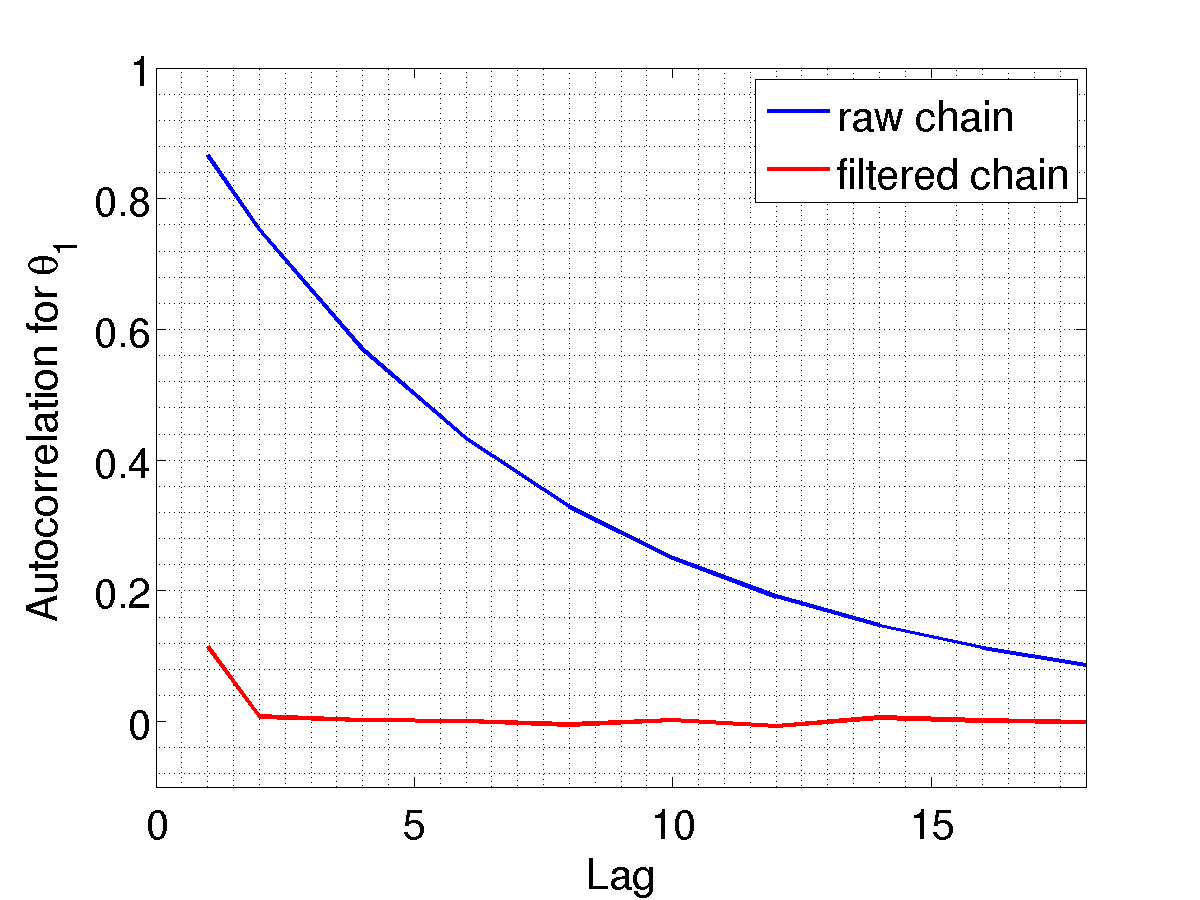
\includegraphics[scale=0.30,clip=true,viewport=0.0in 0.0in 8.0in 7.0in]{figs/paper_plot1.eps}
$~$
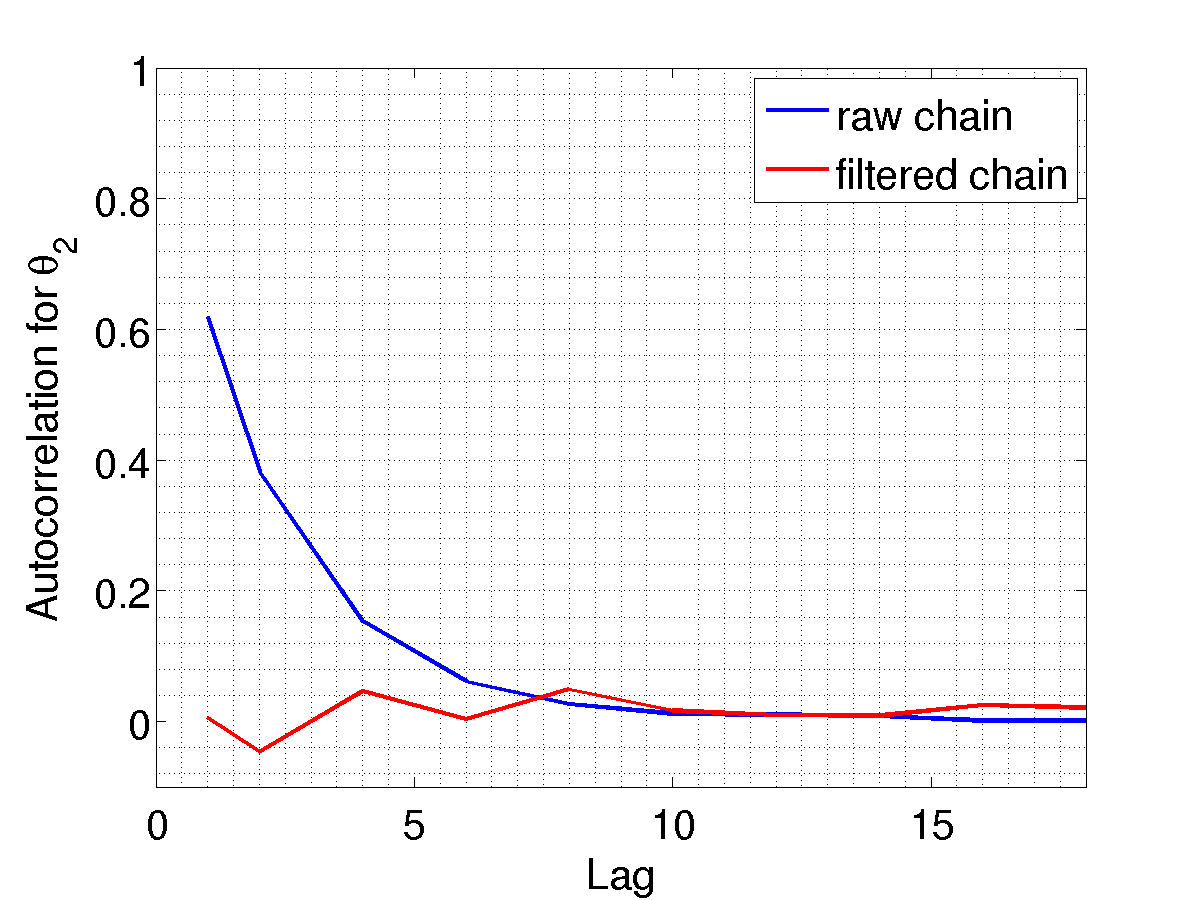
\includegraphics[scale=0.30,clip=true,viewport=0.0in 0.0in 8.0in 7.0in]{figs/paper_plot2.eps}
}
\caption{
Autocorrelation plots obtained with QUESO for the statistical inverse problem.
}
\label{fig-sip-autocorr-plots}
\end{figure}

\begin{figure}[h!]
\centerline{
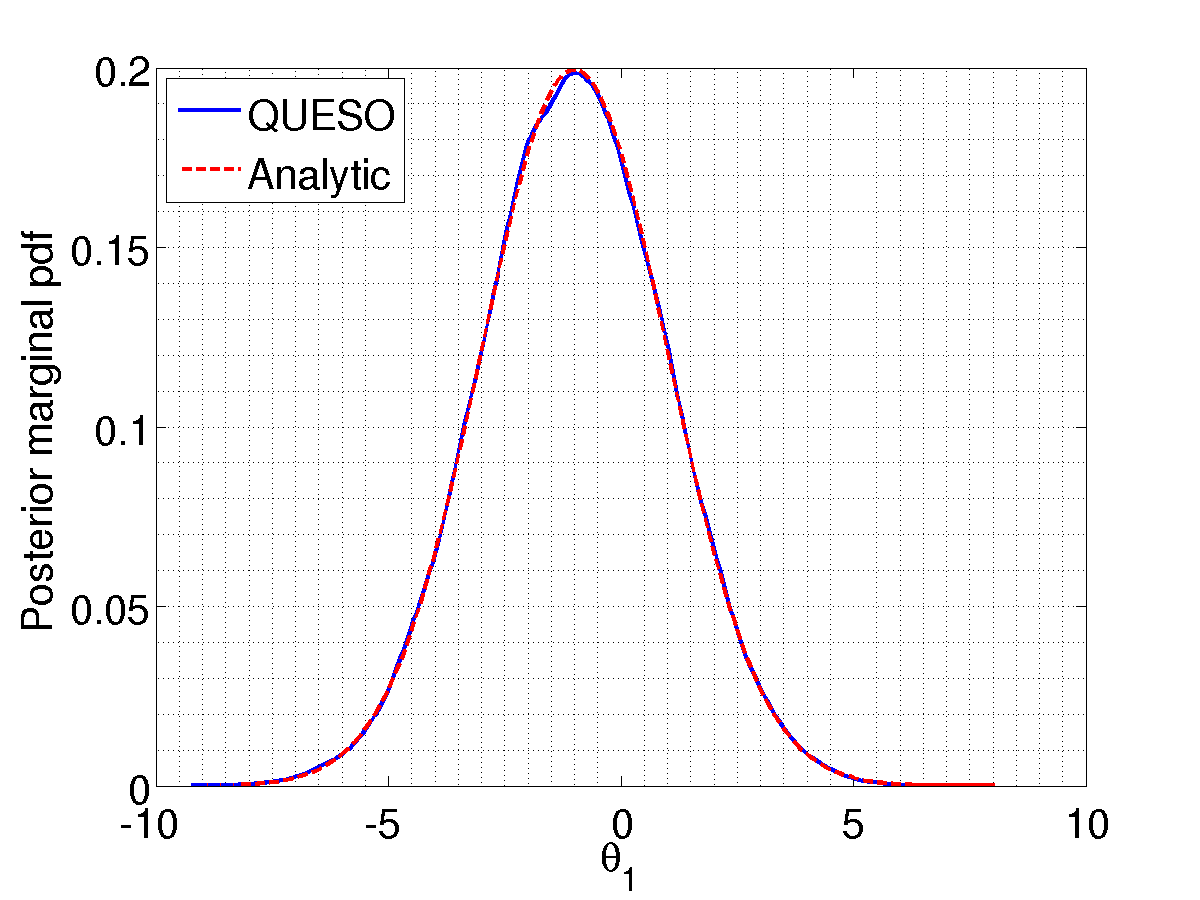
\includegraphics[scale=0.30,clip=true,viewport=0.0in 0.0in 8.0in 7.0in]{figs/paper_plot3.eps}
$~$
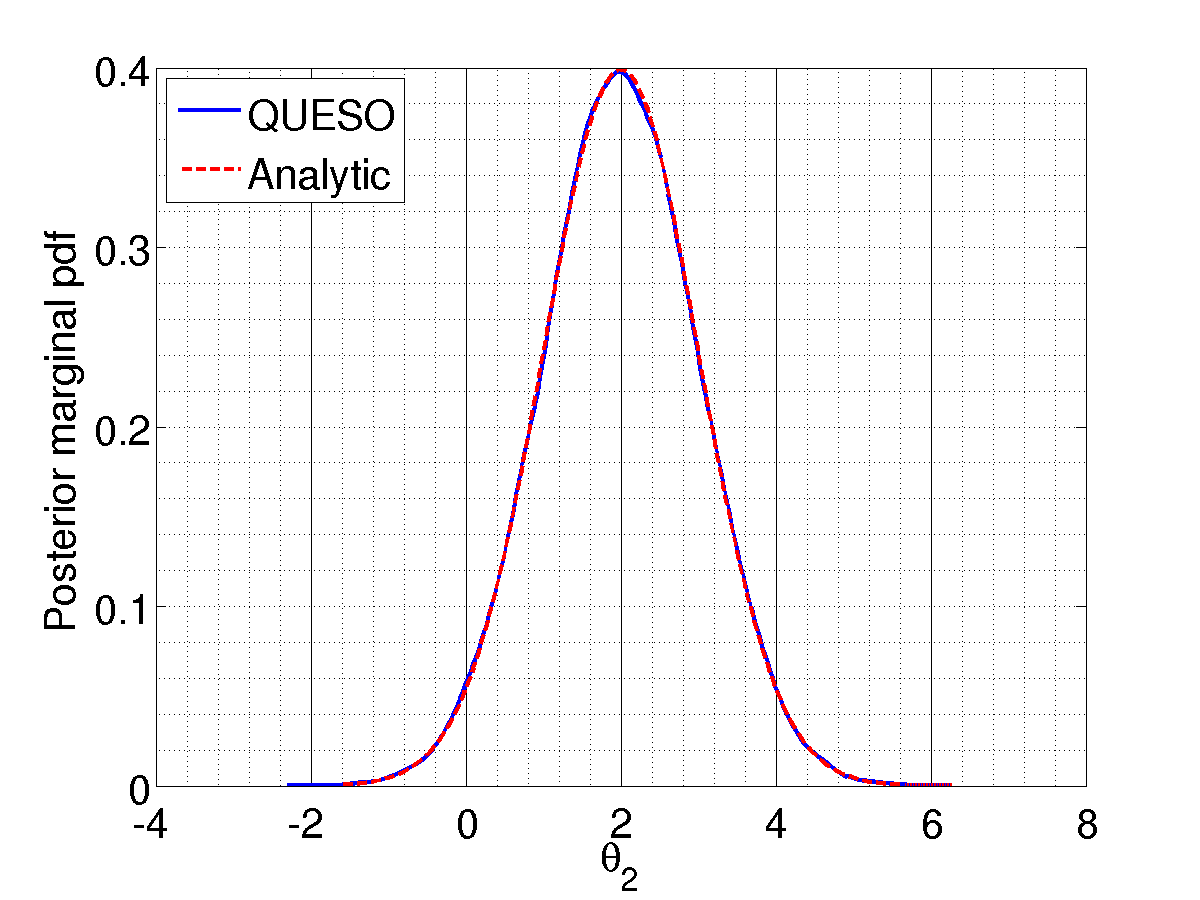
\includegraphics[scale=0.30,clip=true,viewport=0.0in 0.0in 8.0in 7.0in]{figs/paper_plot4.eps}
}
\caption{
KDE plots obtained with QUESO for the statistical inverse problem.
}
\label{fig-sip-hist-kde-plots}
\end{figure}

Finally, correlation matrix and covariance matrices.

\clearpage

\subsection{Results for the Statistical Forward Problem}

\begin{figure}[h!]
\centerline{
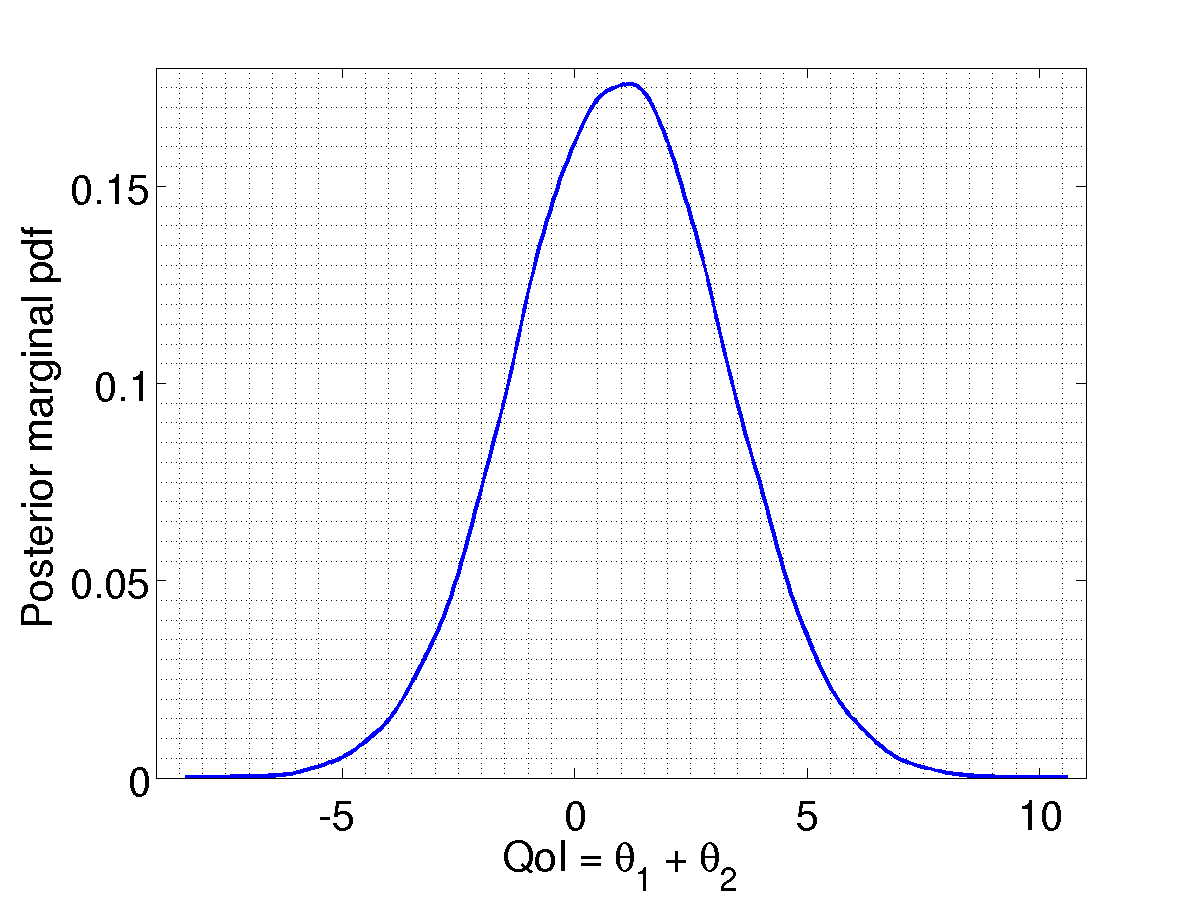
\includegraphics[scale=0.45,clip=true,viewport=0.0in 0.0in 8.0in 7.0in]{figs/paper_plot5.eps}
}
\caption{
KDE plot obtained with QUESO for the statistical forward problem.
}
\label{fig-sfp-hist-kde-plots}
\end{figure}

Finally, correlation matrix and covariance matrices.

